% !TEX root = ../Thesis.tex
\chapter{Implementation}
\label{c:implementation}

This chapter describes an implementation in correspondence to the concepts proposed and ellaborated in chapter \ref{c:concept}. 
These concepts are applied to Polypheny-DB, a particular polystore system.\\
First the current architecture and all relevant components and modules of this system are described. Afterwards each proposition of the concept is adapted
so it can be implemented within Polypheny-DB to enrich it with freshness-aware data management.
This chapter is separated into several building blocks, where each part is necessary to describe the implementation in accordance with the requirements.
It is structured as two main sections. The first addresses the functional requirements (i,iii, iv,) and aims to apply the concepts of Lazy Replication with all its
cross-dependencies., while the second part focuses on introducing the notion of freshness itself, hence aiming to provide the requirements (ii,v, vi).
Finally, all building blocks are gathered and put into perspective to describe an entire lifecycle for freshness within Polypheny-DB. 



Change Data Capture ($\rightarrow section \ref{sec:}$)
Replication Algorithm($\rightarrow section \ref{sec:}$)
Freshness specifications($\rightarrow section \ref{sec:}$)
Freshness evaluation($\rightarrow section \ref{sec:}$)
Freshness constraints($\rightarrow section \ref{sec:}$)


\todo{Talk about each implementation step for the building blocks in general, but if there are deviations e.g. in languages briefly differentiate them with bullet points
and add them to the appendix }




%%%%%%%%%%%%%%%%%%%%%%%%%%%%%%%%%%%%%%%%%%%%%%%%%%%%%%%%%%%%%%%%%%
%%%%%%%%%%%%%%%%%%%%%%%%%%%%%%%%%%%%%%%%%%%%%%%%%%%%%%%%%%%%%%%%%%
%%%%%%%%%%%%%%%%%%%%%%%%%%%%%%%%%%%%%%%%%%%%%%%%%%%%%%%%%%%%%%%%%%



\section{Polypheny-DB}
\label{sec:architecture}


The implementation is based on the polystore system Polypheny-DB\footnote{https://github.com/polypheny/Polypheny-DB}.
In this chapter we briefly describe and illustrate a simplified version of Polypheny-DBs current architecture.\\
This extends the foundations laid out in Chapter \ref{c:Foundation} and sets them in context of the existing system model.


PolyDBMS \cite{polypheny2021}
\todo{Add PolyDBMS cite Love Marriage or Marriage of convenience}

\textit{Polypheny-DB} is an Open-Source project\footnote{https://polypheny.org/} developed by 
the \textit{Database and Information Systems} (DBIS) group of the University of Basel.\\

Polypheny-DB is a self-adaptive polystore that provides cost- and workload aware access to heterogeneous data\cite{poly2020}.

Compared to other systems like \textit{C-Store}\cite{cstore_2005} or \textit{SAP HANA} \cite{hana_2012}, 
Polypheny-DB does not provide its own set of different storage engines to support 
different workload demands.\\
Instead, it acts as a higher-order DBMS which provides a single-point of entry to 
a variety of possible databases like 
\textit{MongoDB}\footnote{https://www.mongodb.com/}, 
\textit{Neo4j}\footnote{https://neo4j.com/},
\textit{PostgreSQL}\footnote{https://www.postgresql.org/} 
and \textit{MonetDB}\footnote{https://www.monetdb.org/}. 
These can be integrated, attached and managed by Polypheny-DB which will incorporate the underlying 
heterogenous data storage engines with their different data structures. 
It is desigend to abstract applications from the physical execution engine while profiting from 
performance improvements through cross-engine executions. 
\\
For incoming queries Polypheny-DB's routing engine will automatically analyze the query and decide 
which store will provide the best response. The query is then explicitly routed to these data stores. 
This approach can be characterized as a dynamically optimizing data management layer for different workloads.\\
Due to its inherent architecture and the possibility to replicate data across different homogenous as well as heterogeneous stores, it is also able to cluster, specific stores 
on a table entity level, although the underlying stores might not support this natively. 
This leverages Polypheny-DB to a data orchestration platform. 



\todoMissing{polypheny support multi-model databsaes for relational, document, graph in memroy ...}

%%%%%%%%%%%%%%%%%%%%%%%%%%%%%%%%%%%%%%%%%%%%%%%%%%%%%%%%%%%%%%%%%%

\subsection{Placements}
Placements are considered to be Polyphenys virtual representation of physical entities.
They act as an abstraction between the polystore layer and the physical representation of an entity. 
Mostly used within the PolyDBMS itself they help to assist the logical routing process of Polypheny-DB.


\begin{description}
    \item [Data Placements] A Data Placement is essentially a virtual representation of the physical entity residing on a given store.
    A store in Polypheny is an underlying physical data storage which is 
    attached to Polypheny-DB.
    All attached stores can be used to hold several fragments of data. 
    During routing decisions stores are automatically taken into consideration if they are designated for the associated data 
    
    It contains information on available columns ($\rightarrow$ Column Placements), partitions ($\rightarrow$ Partition Placements)
    as well as properties unique to this store.
    
    A table can therefore contain several Data Placements with different capabilities and properties. \todoMissing{Image}
    
    are used along the idea of Column Placement. A Data Placement 
        is a representation of table with all placed columns on a specific physical store.
    
        When a table is created on Polypheny-DB it is an ordinary structure placed onto 
        one store. Such a table consists of one to \textit{n}-columns.
        In the context of vertical partitioning a subset of these \textit{n}-columns can now 
        be placed onto another store in form of a \textit{Data Placement}.
        This can either be done by evenly distributing the columns onto these stores 
        or by simply replicating the subset to the second store.\\

    \item [Column Placements] \todoMissing{Image}
    are needed to fulfill the intended flexibility of Polypheny-DB. 
        Column Placements are instances of a column placed on a specific store.
        These placements are the result of the extended vertical partitoning of a table.
        
    Column Placements are instances of a column placed on a specific store.
    These placements are the result of the extended vertical partitioning of a table.
    They are considered unique per column on a cluster.
    
    \todoMissing{Maybe summarize this under Data Placement}
    As already discussed in \ref{sec:part}, vertical partitioning refers to the logical 
    separation of the data structure by columns to obtain logically connected objects throughout 
    the database. 
    Polypheny-DB extends this functionality to vertically partition tables
    column wise, which allows a table itself to be split further into a disjoint 
    set of columns. This extension provides the functionality to place columns 
    rather freely on a store without replicating the complete table. 
    Although these columns are logically bound to a table there is no need 
    to replicate the complete structure to a desired store. In some cases 
    this does not only result in an optimized access of the data part but 
    also saves data overhead on the specific store.\\
    This functionality enables Polypheny-DB to adapt the data structure to continuously 
    varying use cases.\\

    \item [Partition Placements] Due to the partition function NONE every table entity inside Polypheny-DB is considered to be partitioned.  Hence consisting only of one partition.
    Additioanlly, Polypheny suppports the most common partition algorithms like HASH (), range or list(). 
    
    A Partition Placement is 
\end{description}



%%%%%%%%%%%%%%%%%%%%%%%%%%%%%%%%%%%%%%%%%%%%%%%%%%%%%%%%%%%%%%%%%%


\subsection{Query Routing}

Routing or cache plan optimizat execute

\todoMissing{Image}
Since every query has to go through the abstraction layer to guarantee correctness 
and consistency, Polypheny-DB can consult the systems \textit{Catalog} to retrieve the
location of all relevant data. This is done by gathering all 
\textit{Column placements} needed by the query.\\ 
If the requested data indeed happens to be distributed
on several stores. The central routing engine will join all relevant and distinct 
placements to construct the result set. Hence, the query is always routed to stores which 
hold relevant data.


Since partitions are mere logical identifiers there main usage is to locate data fragments or the location where a query should route a statement to.
One physical table can therefore hold several partitions.
During routing if a partition has been identified it is checked for every store involved whether it contains and associated partition placement.
Although, this routing method is quite fast there are several problems concerning the separability of data.
This imposes for one the difficulty to retrieve data belonging to exactly one partition out of a table which contains several partitions and secondly difficult 
to migrate data from individual partitions to another store.\\
Since it is rather complex to extract all relevant partitions needed for a specific query especially when combining vertical and horizontal partitioning
the concept of \textit{Worst case Routing} was introduced.\\
This routing mechanism aims to improve performance, when the process of identifying the correct partitions for a query would be too complicated and 
therefore also reduce the overall performance.   
This is the reason why currently, a \textit{Full Placement} has to be enforced for all three Partition Managers to support the functionality of worst case routing.
A Full Placement in that sense refers to a placement on a store which contains all partitions of a specific table and can therefore be used as a fallback scenario.

However, due to the adjustments to partitioning including the new Partition Placements which are represented by their own individual physical tables, the constraint imposed by logical 
partitions and therefore the necessity of a full placement per table can be removed.\\
Queries are  now able to flexibly combine vertical and horizontal partitioning to truly leverage the power of Polypheny-DB.
The routing for SELECT-queries is now simplified since it aims to find for each partition all requested columns by 
joining Column Placements per partition first and then applying a UNION over all accessed partitions to build the required result set.




\subsection{Concurrency Control}

Given Polyphenys current architecture all incoming queries has to be delivered through the poly-layer, acting as a central instance.
Since we assume that there is no direct interaction with the underlying systems there is no immediate risk of inconsistencies. 
This allows the utilization of SS2PL to handle concurrency control only within Polypheny-DB for correct isolation treatment.






%%%%%%%%%%%%%%%%%%%%%%%%%%%%%%%%%%%%%%%%%%%%%%%%%%%%%%%%%%%%%%%%%%
%%%%%%%%%%%%%%%%%%%%%%%%%%%%%%%%%%%%%%%%%%%%%%%%%%%%%%%%%%%%%%%%%%
%%%%%%%%%%%%%%%%%%%%%%%%%%%%%%%%%%%%%%%%%%%%%%%%%%%%%%%%%%%%%%%%%%


\todoMissing{Maybe rename?}
\section{Lazy Replication}
\label{sec:lazy_replication}

This section discusses all implementations along with the introduced components and services to establish 
multi versioning and the possibility to refresh specific replicas. This serves as a foundation in order to use those distinct versions
to be used within query retrieval. Which again shall help to reduce the overall latency of the system by allowing a mixed worklaod to exist in parallel.

\todoMissing{In correspondence to the section \ref{sec:propagation} update propagtion in concept we focussed on implementing the CDC approach ($\rightarrow$ \ref{sec:algo}) 
as well as the on-demand approach using Priamry Snapshot Copy ($\rightarrow$ \ref{sec:manual_refresh}))}


\subsection{Placement Versioning}

As we have established in section \ref{sec:data_replicas}, the existence of multiple data replicas are fundamental in distributed systems to even provide the 
possibility of a trade-off between latency and consistency. These versions essentially allow load balancing requests among all suitable replicas to effectively 
use the entirety of the system. This does not only enable one to distribute the load evenly across the landscape, hence increasing availability
but also defines how many of these replicas need to utilized jointly to enforce the desired consistency constraints.\\

As the name might suggest, a multi-version database would be ideal and the obvious choice for such an approach.
These databases will automatically generate a new version per data object for each modification. 
Due to their properties we would immediately have the information on the validity-interval of the version, its update time as well as predecessor and successor versions.
This would directly allow us to utilize these versions on freshness-related queries. But, this would also imply the utilization of MVCC.
However, as stated in \ref{sec:concurrency_control} multi-version databases automatically tend to have larger data footprints, due to persisting  
redundant and even obsolete data.
Howeever, polystore systems already suffer from a larger data volume, given the redundant data storage across severall stores.
Finally, aforementioned, Polypheny-DB currently only supports SS2PL for its concurrency control.
Since we require to have equally converging states for our outdated versions \textit{(iv)}, we need a serializable execution that can be applied to 
the underlying stores as well.
Although, MVCC reduces common blocking scenarios and allows write- and read-operations to be executed in parallel, 
it cannot reliably produce a serializable execution order of all operations among all participating stores.
That is why we remain with SS2PL and refrain from using the automatic versioning provided by a multi-version database.\\

However, as already mentioned in chapter \ref{c:concept}, multiple versions are automatically created when using a lazy update propagation. 
This will directly loosen the constraints, impossed on replicas to update. 
The update in these cases will then only be targeted towards the primary replicas, drastically reducing the reponse time of a write-operation,
but lowering the consistency at the same time.  \todoMissing{Besserer Übergang}
Furthermore, to provide freshness-awareness as well, we do not only require several versions for updates to be applied quicker,
but also be able to actually utilize these versions to efficiently operate on the entire system.
These versions therefore also allow us to compare and find suitable candidates in freshness related queries.\\

Fortunately, polystore systems and especially Polypheny-DB is inherently distributed, automatically providing potentially multiple replicas.
Although they might be distributed or replicated, resulting in redundant data storage, Polypheny-DB allows to create multiple data placements for an individual entity. \todoMissing{Besserer Übergang}
The data placements described above can therefore be considered as an individual replica or version for a corresponding data item as referred to in the concept.
Therefore to enable Polypheny-DB to retain different levels of freshness we need to allow our routing process
to only target a subset of all placements for primary update transactions. The remaining placements will therefore autoamtically become outdated. 

However, since partition placements logically refer to the physical entities that actually persist the data and 
read-only queries typically benefit directly from data partitioning (see \ref{sec:part}), Polypheny-DBs partition placements 
are suitable candidates to base our freshness awareness on.


\begin{figure}[t]
    \centering
    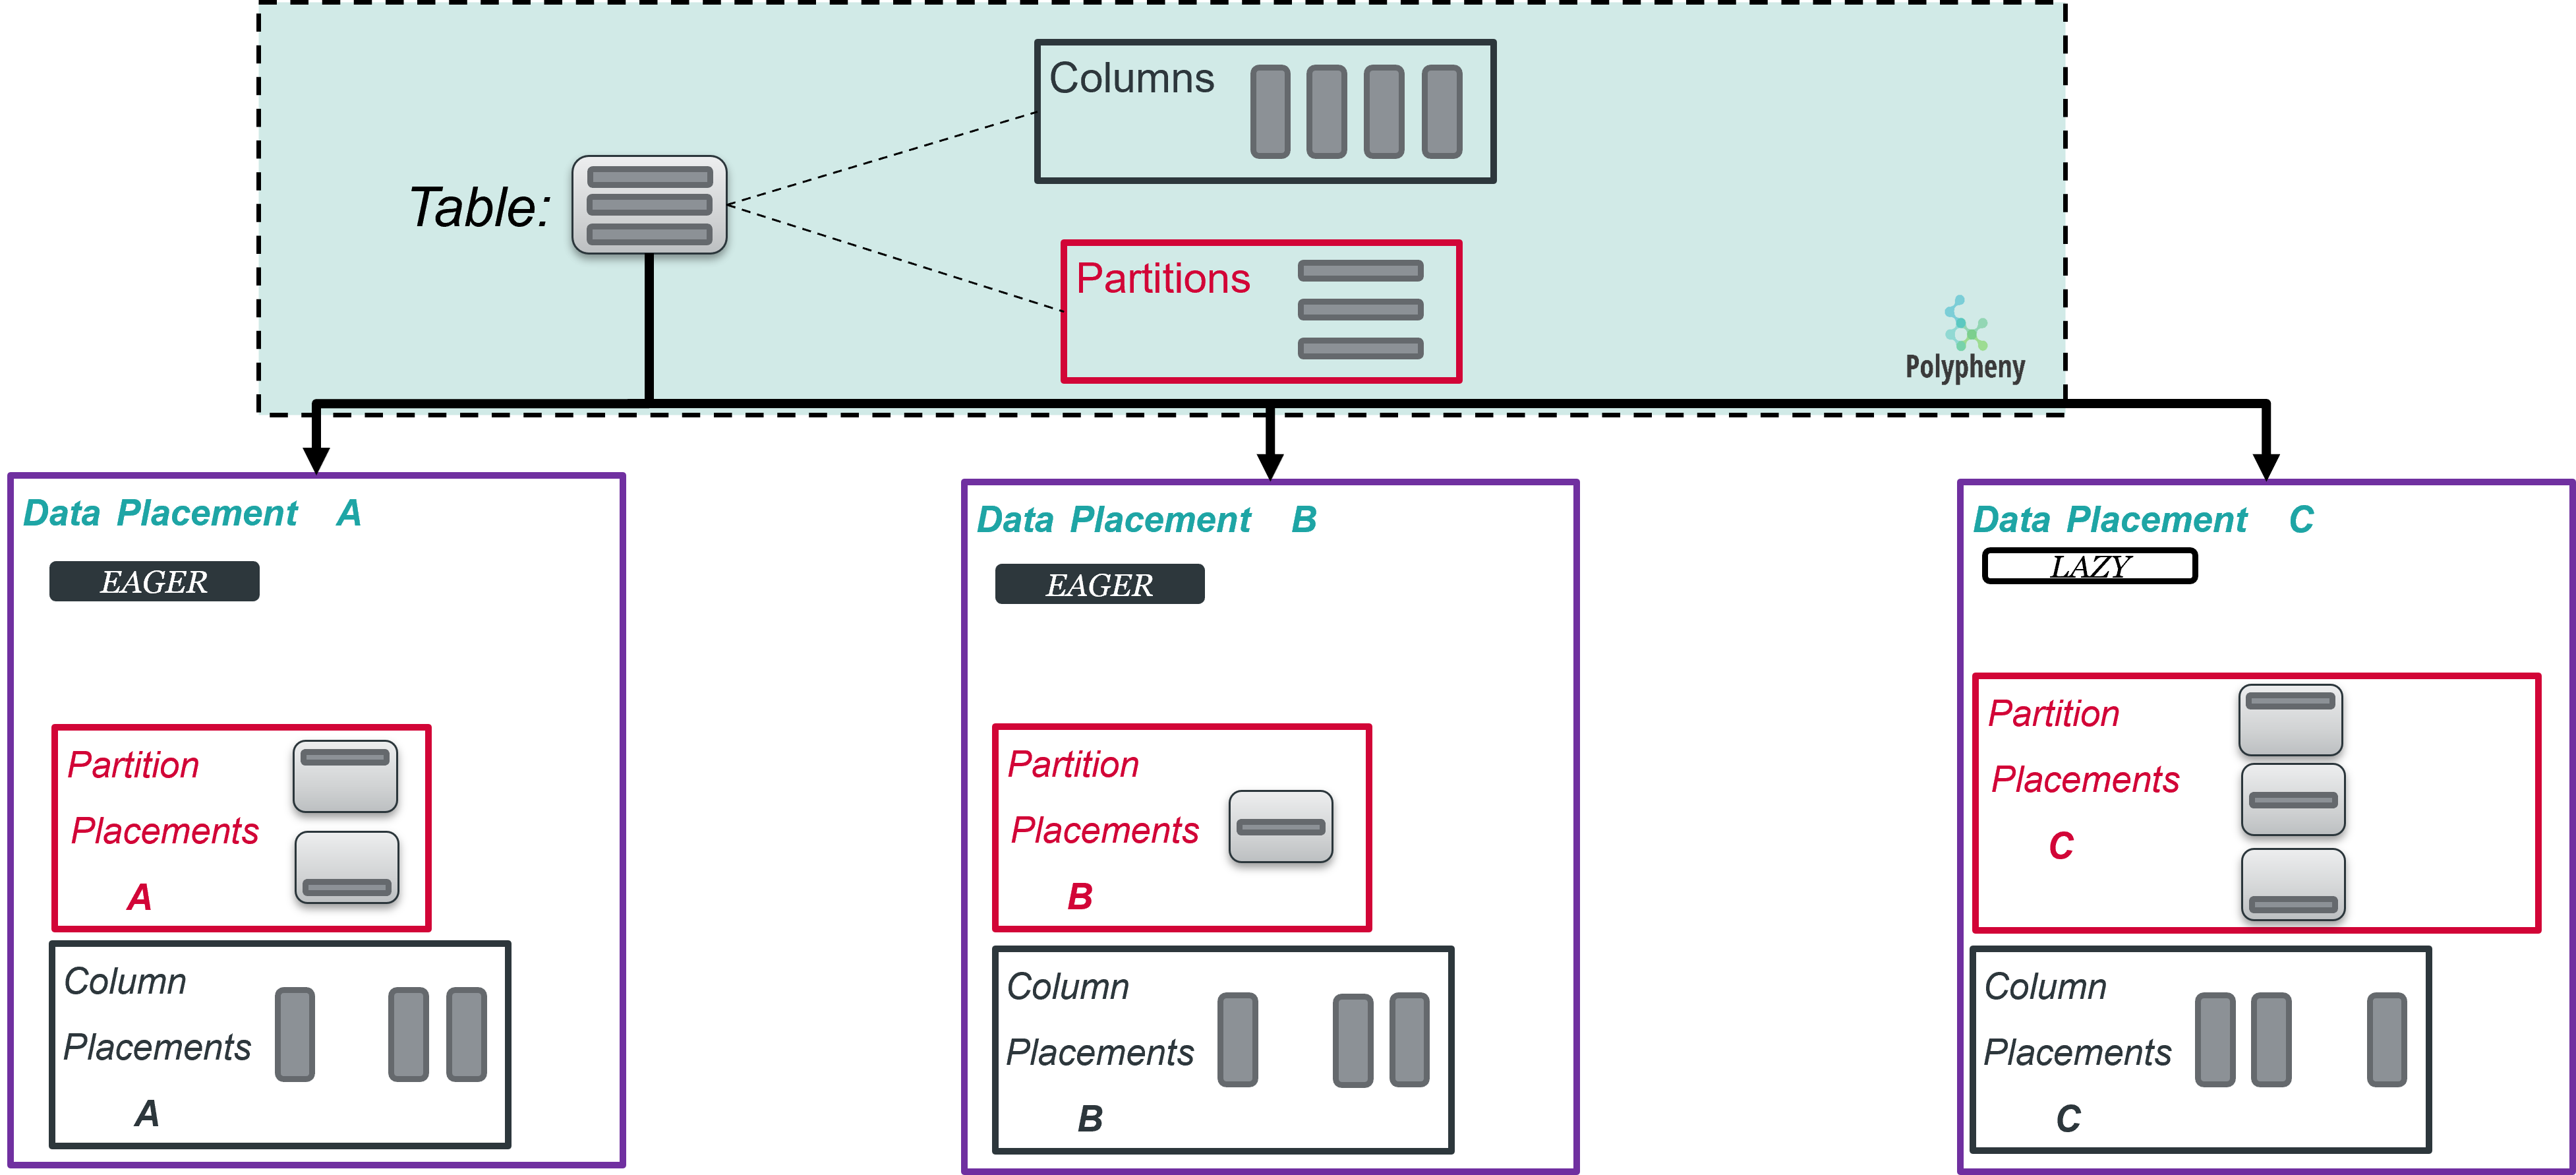
\includegraphics[width=0.7\textwidth]{Figures/entity_placements_replication.png}
    \caption{Entity alongside all its physical placements}
    \label{fig:placements}
\end{figure}



%%%%%%%%%%%%%%%%%%%%%%%%%%%%%%%%%%%%%%%%%%%

\subsection{Replication Strategy}
\label{sec:strategy}

In order to reduce the update time per write-operation and increase the performance
of OLTP workload, we need to enable Polypheny-DB to identify placements that need to receive updates immediately. 

To allow the routing process to differentiate between such placements,
we need the possibility to label data placments on how they are going to receive updates. This is defined as the \emph{Replication Strategy} $\Gamma \in \{EAGER,LAZY\}$.
\emph{EAGER} means that DML operations are applied at once, while \emph{LAZY}
allows data manipulation to be deferred, resulting in outdated data.\\


Although, we defined that we will base the freshness evaluation on partition placements, we implemented the strategy per data placement. 
As introduced in the beginning of this chapter, partition placements inherit their information from its corresponding data placement.
Although they receive there updates independently their properties are defined within the parent placement. 
Therefore, it is sufficient to configure the data placement to achieve an intended state of the subordinate partition placements.
Such that a partition on a given store can either be updated enitrely eagerly or lazily. 

\todoMissing{integrate SYNC and ASYNC}

%Since the locking within Polypheny-DB is done logically within the polystore layer and locks the entire table.
Since we want to establish the freshness comparison based on each individual partition placement, the locking mechanism
has been adapted to allow locking on partition level rather than on a table-level. 
This allows for a much finer level of detail and increases the degree of parallelism. 

Can be used to selectively define which data placement shall be updated lazily.
The replication strategy can therfore be directly defined as:
\begin{lstlisting}[language=sql]
    ALTER TABLE tableName MODIFY PLACEMENT ON STORE storeName WITH REPLICATION ( LAZY | EAGER );
\end{lstlisting}

This replication strategy is added as part of the newly added data placement properties. Since Data Placements inherently carry the information, what column and partitions reside
on a given store, they were extended to now also hold information on data placement specific properties.

When a placement is created without any replication strategy, it will automatically be labeled to receive updates eagerly.\\
This allows us to flexibly define the strategy per data placement, considering all necessary constraints to ensure the conssitency and integrity of the data (see \ref{sec:constraints}).


%%%%%%%%%%%%%%%%%%%%%%%%%%%%%%%%%%%%%%%%%%%


\subsection{Replication State}
\label{sec:states}

Since the replication strategy is bound to an individual data placement we still need the possibility to 
define how the actual partition placements, that hold the data, will behave in certain scenarios and will consequently be processed.
We therefore introduce the \emph{Replication State} per partition placement.\\

This replication state is logically bound, and directly influenced by the replication strategy defined within a data placement
and can be differentiated into three states that define the intended state of a given partition placement. 
\begin{description}
    \item [UPTODATE] Is automatically set within a partition placement, when the parent placement is configured to receive updates eagerly.
    This cannot be changed by any user. It does also not refer to the current state of any data object, meaning that an lazily updated placement can become up-to-date overtime.
    Allthough this is possible in terms of the received update, it is not respresented using these states. They rather impact the behaviour and handling during processing.
    
    \item [REFRESHABLE] Initially this is configured when the corresponding data placement receives updates lazily. This allows the partition placement to actively receive 
    individual updates by a replication algorithm. A refreshable state can be automatically and manually transformed into an \emph{INFINITELY OUTDATED} state.

    \item [INFINITELY-OUTDATED] This state is specifically marked, to stay outdated and not receive any updates. This can either be done manually, because a user may want to
    retain an item with a given version, hence surpressing the automatic update replication on this node. Additionally this can be set autoamtically by the system, 
    if either the entire store or the system is not available anymore. This can be caused due to an unexpected outage or simply because the replication algorithm has 
    numerously failed to apply updates, indicating an error. Given certain prerequisites it can be manually transformed back into an \emph{REFRESHABLE} state.

\end{description}

The distinction between these cases is necessary, to allow treating partition placements on a given store differentely. 
Otherwise if one partition placement would be automatically labeled as \emph{INFINITELY OUTDATED} the entire data placement could be refreshed anymore.
Therefore they are handled and considered independently.

Although, this state is required for internal processing of individual partition placements, the manual specifcation of this state is still targeted to an entire data placement.
Since the internal partitioning should be rathe ruser agnostic one should only be able to specifiy this per data placement. 
As with the replication strategy, the changes are then propagated downwards to all linked partiton placements. 

They have a dependency that refreshable can be set to INFINITELY OUTDAED and vice versa, however UPTODATE can only be influenced by the replicaiton strategy.
Trying to change this manually will result in an error since it is controlled by the system.
\todoMissing{flowchart?}

Placements containing \emph{REFRESHABLE} 

\begin{lstlisting}[language=sql]
    ALTER TABLE tableName MODIFY PLACEMENT ON STORE storeName WITH STATE ( REFRESHABLE | OUTDATED );
\end{lstlisting}
OUTDATED referring to INFINITELY OUTDATED,  by explicitly labeling it as outdated it will suspend all update propagation towards those stores.

Furthermore each Partition Placement is enriched with the most recent update information to support various freshness metrics.
This update information contains insights such as the id of the last comitted update transaction, the corresponding commit and update timestamp as well as the number of 
modifications that 


Therefore, we propose to define the outdatedness on the state of a specific partition placement.
Although the entire data placement, could be labeled as outdated or rather receive updates lazily, some of 
these partitions could already be up-to-date again, while others still remain outdated.


%%%%%%%%%%%%%%%%%%%%%%%%%%%%%%%%%%%%%%%%%%%

\subsection{Change Data Capture}
\label{sec:cdc_impl}

Influenced by the replication strategies the routing process is now capable of differentiating between placements needed to be updated immediately or asynchronously. 
When processing a DML-operation, the router can identify for a given entitiy if it contains at least one placement that is updated lazily.
If this is true it will capture all executed changes within a \emph{Change Data Object} to be later applied on these placements. 
Disregarding the operation type $\in \{INSERT,UPDATE,DELETE\}$, it contains information on all logical partitions that have been involved, 
the executed operation, as well as the current statement and transaction id. For \emph{DELETE} and \emph{UPDATE} operations it also stores additional information on possible filter 
conditions. Each statement within a transaction can have at most one of these objects and refers to one operation to be executed.\\

After creation this object will be added along its statement id to a preliminary \emph{capture-queue} within the \emph{Change Data Collector}. 
As visualized in \ref{fig:capture}\todoMissing{Add illustration of hashtable in data colelctor identifiyng transaction to stateemnt.} this capture-queue is represented as as hashtable for 
faster retrieval, and maps a transaction to a list of statements that require change data capture. 
These statements are stored with respect to their execution order within the parent transaction.
Each statement inside this structure is attached to its respective \emph{Change Data Object}.\\

To be able to apply operations directly to the outdated replicas, they need to be converted into basic operations that can be applied to a prepared statement.
Therefore they are captured before they are executed but after they have been evaluated.\\
Since not all stores provide the same functional capabilities, we can leverage the polystore-layer to pre-compute certain calls before applying them to the underlying stores.
Typical functions that are not uniformly provided are e.g.: \emph{CURRENT\_TIME} or \emph{TIME\_NOW}. This allows storing the actual values that are executed on the store,
hence saving execution time during update propagation.
During runtime of any given statement the actual evaluated data values are then injected into the object stored within the capture-queue.\\
The benefit of this structure is that as soon as the transaction commits, the \emph{Change Data Collector} is notified, streaming all objects in correct execution order
into the \emph{Replication Engine}, where they will be transformed into individual \emph{Replication Objects} and finally queued to be propagated onto outdated placements. 
Since the registration is done during the commit, we are sure that any pending changes will be available for distribution once the transaction has been commited.



%%%%%%%%%%%%%%%%%%%%%%%%%%%%%%%%%%%%%%%%%%%

\subsection{Lazy Replication Engine}

A \emph{Replication Engine}, contains the core functionality that transforms capture objects into distinct replication objects and 
pipes them to specific execution engines.
The \emph{Lazy Replication Engine} is a specific implementation of the general replication engine and enhances it with several additional capabilities targeting
the lazy replication strategy. This engine essentially provides the CDC approach proposed in section \ref{sec:refresh_operations} and is influenced by the 
change data capture service of section \ref{sec:cdc_impl}, to apply changes operation-wise to designated targets.\\

During commit time of a transaction, all corresponding \emph{Change Data Objects} will be first transformed into distinct \emph{Replication Objects}. Other than
the generic change objects these are restructured and specifically tailored to specific operations and designated targets. During transformation the engine retrieves all 
relevant placements that are currently defined to receive updates lazily. Then for each of these target placements an individual replication object is generated, allowing to 
replicate changes independently from each other. These transformed objects are then added to a \emph{Global Replication Queue} which concludes the change data registration process.\\


The engine itself is decomposed into the following services that jointly allow an asynchronous execution of modifications within Polypheny-DB. 

\begin{description}

    \item[Replication Data Object] This object contains all information, necessary to re-create a statement which is equivalent to the orginal one,
    that has already been executed on the primary placements. 
    Therefore it keeps information on the orginal transaction, its commit time as well as the operation type and the data to be delivered. 
    This is further enriched with a list of all target partition placements that shall receive this modification. The list of targets is generated
    at the time the initial update transaction has been committed and changes have been queued. In order to avoid storing data redundantly, this data object 
    is centrally stored and only referenced by depending replication objects, disregarding the number of placements that shall receive a given DML-operation.
    This data is kept as long as there are replication objects depending on it for executing their replication.


    \item[Global Replication Queue] 
    
    \begin{figure}[t]
        \centering
        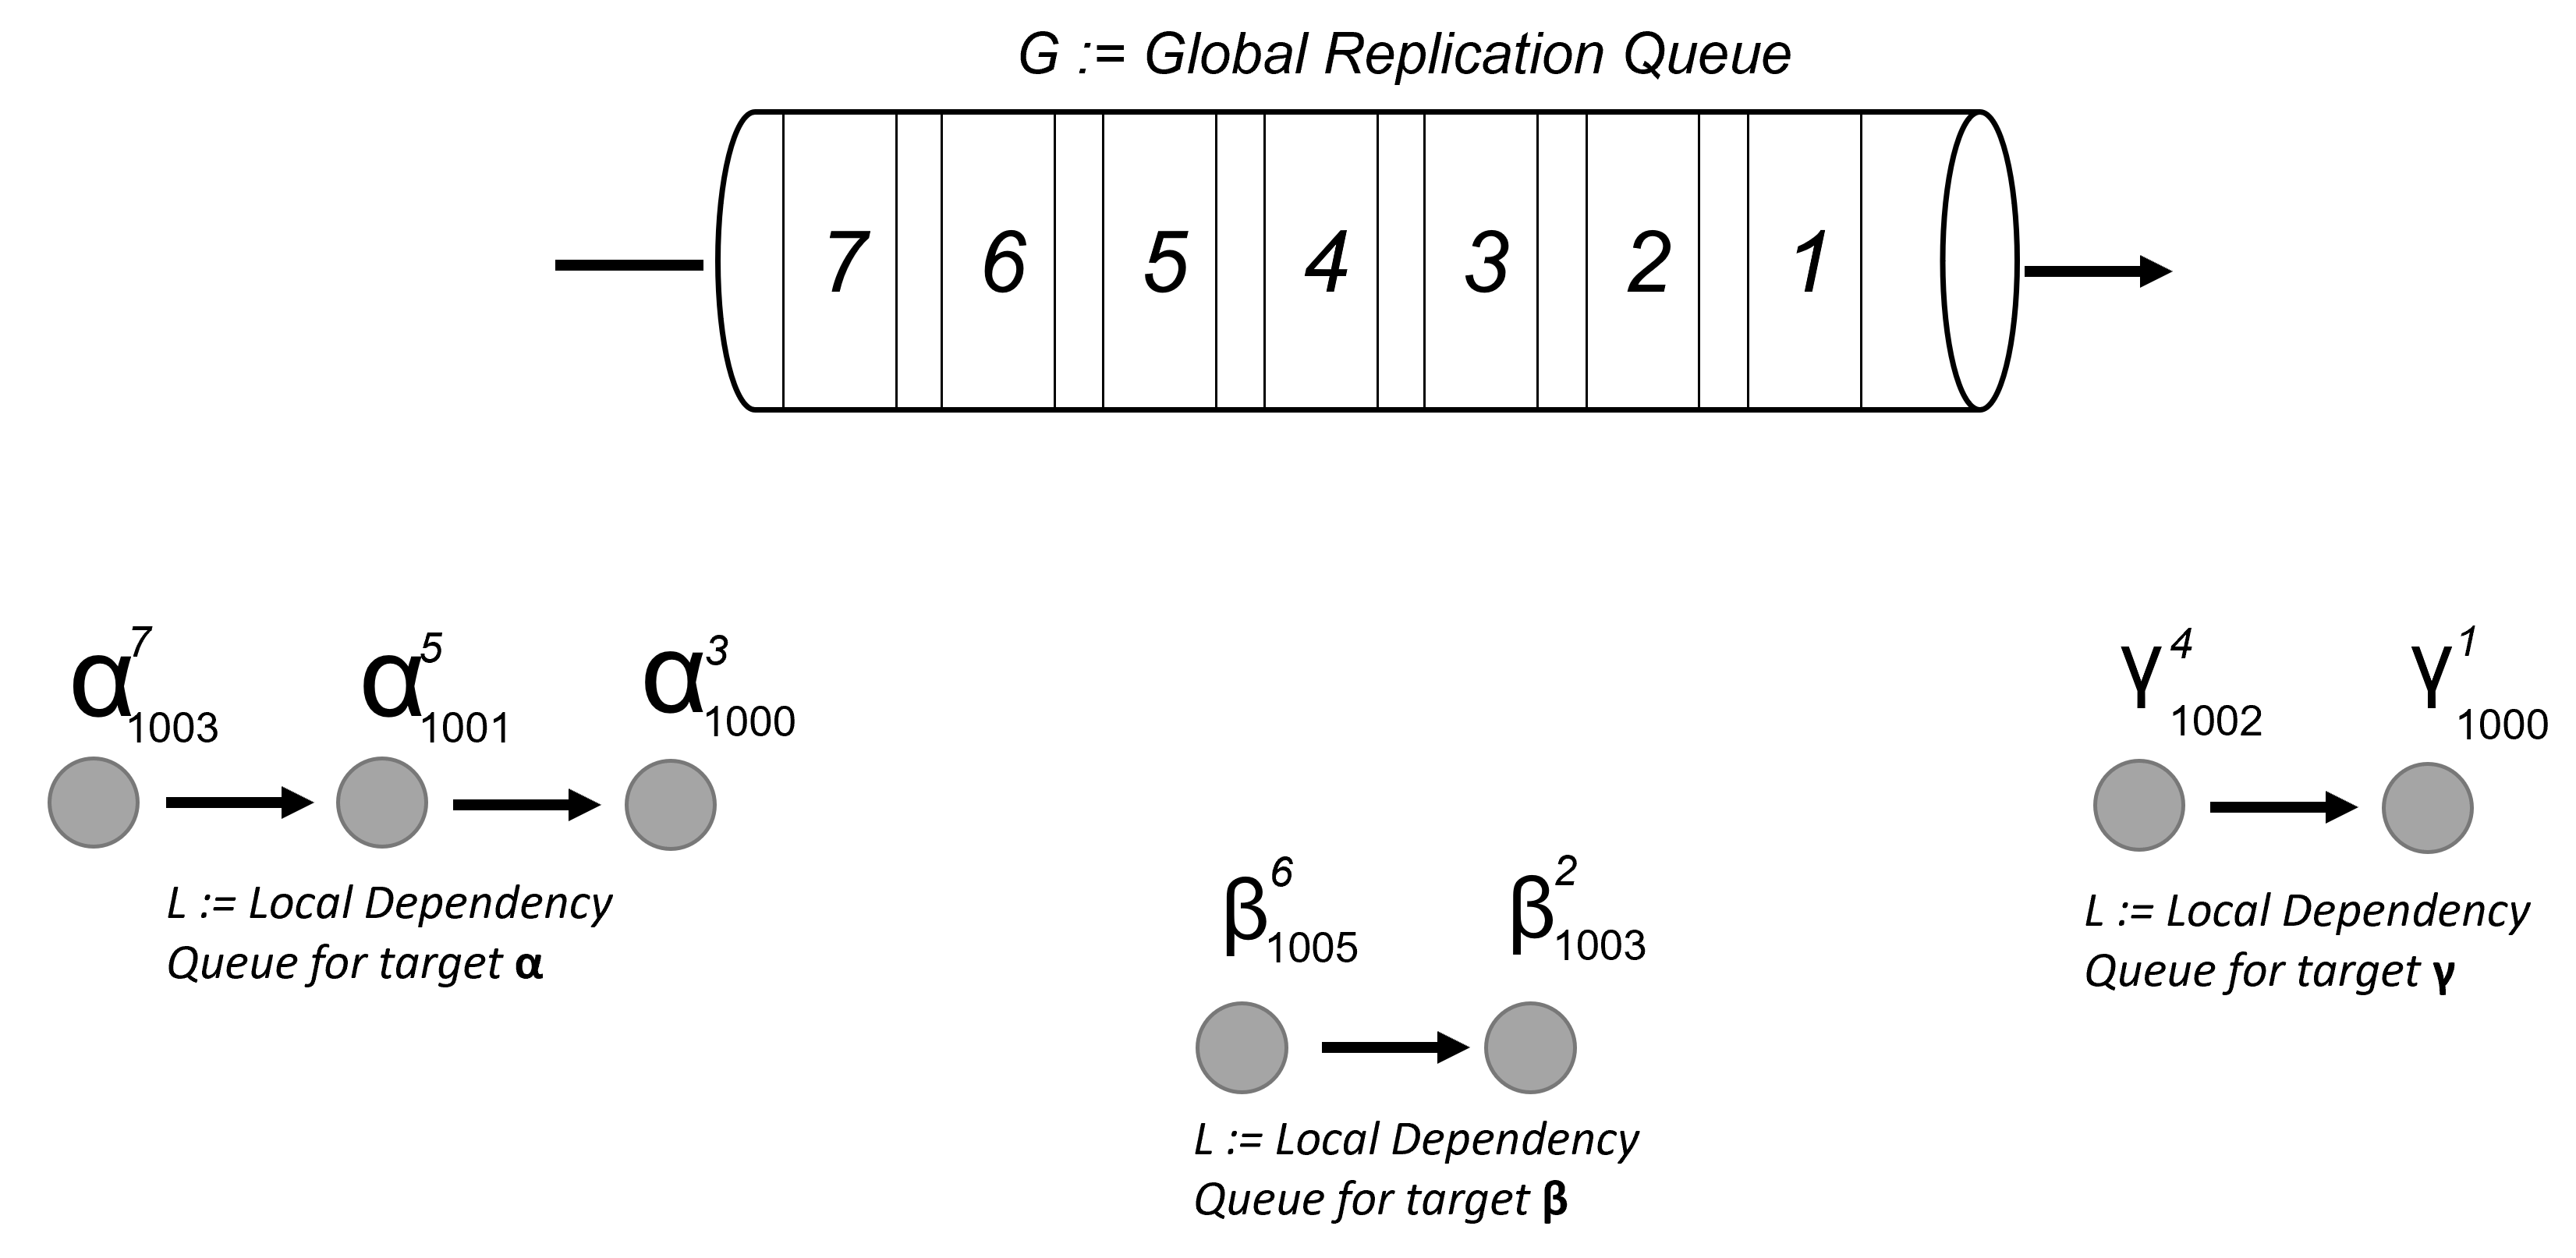
\includegraphics[width=0.8\textwidth]{Figures/Queue.png}
        \caption{Association between global replication queue and local dependency queues}
        \label{fig:queue}
    \end{figure}

    This queue is the core component and the inherent driver revolving around the lazy replication approach. 
    It contains individual replication IDs which correspond to replications targeting exactly one partition placement at a time.
    As depicted in figure \ref{fig:queue} it is represented as a FIFO queue receiving new replication IDs that are registered through the \emph{Change Data Collector} 
    or are rescheduled by \emph{Replication Workers}.\\
    Each replication event within this queue is therefore defined as $x_{z}^y$, where $x$ represents the designated target partition placement, $y$ a global
    replication id uniquely identifiying a specific replication object and $z$ a reference linking to the actual replication data. 
    Since our replication engine should replicate the data operation-wise, each event within the queue corresponds to one operation associated with one target partition placement.
    Therefore each event can be applied independently. Since the priamry transaction can only be committed when teh data to be replicated has been added to this queue,
    it stores the replication events in-memory.

  
    \item[Local Dependency Queue] This queue is defined per partition placement containing pending updates that are yet to be replicated. 
    Since all updates need to be delivered in the same order as they have been applied on the primary replica, they depend on each other. 
    Although labeled and represented as a queue, the entries are saved as an DAG. Where each replication event depends on its predecessor to be executed first.
    Since the entries within this queue are not added concurrently and are ordered according to their execution order, we are certain that the imposed dependency
    reflects the original execution order. Therefore this queue is used as an utility to enforce constraints on all intermediate steps ensuring that operations are applied 
    in correct order, that all replicas converge equally towards a given target. 


    \item[Replication Worker] These workers are an essential part of the replication engine since they continuously process events from the global queue 
    and initiate the execution. As soon as a worker thread has finished processing a replication, it will tak the oldest item from the global queue. 
    Before starting the replication process, it will make sure that this is indeed the next replication to be executed based on the dependency constraints
    within the local dependency queue. If the replication event is not the next to be executed, the worker will re-queue the event, to be proccessed later.
    However, if all prerequisites can be verified a dedicated refresh-transaction is started.
    The one operation is passed on to the \emph{Data Replicator} which will then actually execute the statement on a given target.
    After successful termination, the worker will remove this dependency form the local queue as well as from the replication data. \\
    Based on the current load and the number of pending replications on the system, these workers will be scheduled as needed, allowing to dynamically scale as the system grows.
    Since the \emph{Local Dependecy Queue} always will ensure the correct execution order a concurrent processing of the replicaitons is possible.     
    


    \item[Data Replicator] Is implemented as the actual execution engine which will recreate and execute a captured operation. 
    It is invoked by the replication workers, passing a replication event together with a reference to the corresponding replication data.
    For the Lazy Replication Engine, it will receive one operation per target placement. 
    This has the advanatage that we can now decide based on the targets current placement structure, how to reconstruct the statement. 
    Because this is done right before execution, it shows the benefits of capturing the entire object instead of the statement to be executed per placement. 
    Since this target could have been altered since capturing, it could now have a different set of columns.



    \item[Update Metadata] Since data is essentially stored on physical entities, represented by the internal partition placements, we extended these objects 
    to contain information on general update statistics relevant for this particular placement. These information will be updated at commit time of a write-operation.
    For eagerly replicated placements this is the priamry transaction, for lazily replicated however the refresh transaction.
    This enables the system to use this update information to essentially retrieve the current state of the data, represented by the commit timestamp
    and the numer of updates this partition placement has already applied. Allowing us to use those metadata to compare different versions against each other.
    \todoMissing{Maybe illustration}

\end{description}



With all these services the replication engine is able to process multiple replications at once, while ensuring the correct execution order and stability
for each replication to be executed. 
Since all operations are propagated atomically within one transaction we do not need to worry about a rollback of a refresh transaction or provide complex undo-operations 
to remove those changes. Therefore, these replications can be applied independently per target partition placements and do not interfere with each other, 
allowing for a high flexibility.
Furthermore, it does not only replicate the captured modififcations it provides a fault-tolerant approach as well. 
Since Polypheny-DB consists of multiple attached stores that might suffer from outages or local failures, replications might fail.
However since the replication data is centrally stored and is only removed when all dependent replications have been executed, 
a replication event that coninuosuly keeps failing will uneccessarly occupy worker threads and waste storage resources to preserve the data.
Therefore a centrally configured \emph{Fail Count Threshold} is introduced. Everytime a replication fails, the responsbile worker thread will increase the \textit{fail counter} 
of a given replicaiton object. If it reaches the threshold the replication will be removed from the queue entirely. 
Furthermore the traget will be removed from the engine by deleting all remaining local replications for this target as well.
Consequently this particular partition placement will be suspeneded for active data capturing and marked as \emph{INFINITELY OUTDATED}.\\

Due to the architecture of the queue, we can only get an event at the top of the queue. This increases the difficulty to remove all associated replications 
for a target placement at once. However since workers will validate if replications can even be executed and can therefore identify suspended targets, they will
automatically cleanse the queue from unwanted replications, without expensively removing each item within the queue.\\

Moreover contentions can also occur directly within Polypheny-DB, if there are too many pending updates, waiting to be replicated.
Despite the scaling capabilities of the workers the load on the system might still be too high essentially affecting the main operation on the system.
However part of the defined requiremnts are 
Therefore we have enriched the configuration to globally enable or disable the replciation distribution. In constrast to labeleing data placements as outdated, 
and removing all pending replications for ever, we can now allow to temporarily stop the replication and only continue to capture modifications. This can help the system
to adapt to high load situations by focusing on the core funcitonality.\\

However despite this ability to remain operational during failure situations, the utilzed queues within the engine are still only stored within main memory.
Although this increases the overall commit time of a transaction it results in a loss of all captured data that has not been applied yet, as soon as the system 
shuts down for any reason. Since we rely on the fast registration process to commit the primary transaction as fast as possible we need to mitigate this behaviour.
Since we always know which placments are updates lazily, the replication engine can immediately provide two different mechanisms that can be centrally configured. 
The first approach is simple and fast to execute. It gathers inforamtion on all placements that need to be updated lazily. It can automatically mark them as INFINITELY OUTDATED, 
and therefore suspending any more replications. Users can either choose to update the system manually or refreshing is on read as proposed in \ref{sec:refresh_strategies}.
The second approach approach however results in a much slower startup time by refreshing all placements first, before the system will even start.


- Queueing process as flowchart
- replication process as flowchart



%%%%%%%%%%%%%%%%%%%%%%%%%%%%%%%%%%%%%%%%%%%

\subsection{Automatic Lazy Replication Algorithm}
\label{sec:algo}

\todo{Uses the provided change data capture approach}

The goal of the entire lazy replication approach is providing a scalable and fault tolerant approach to distribute the data for each placement onto the designated stores.
Therefore, the algorithm as depicted in figure \todo{ref image of flowchart}, aims to provide a cost-efficient approach to replicate the change data without increasing 
the overhead of the system and impacting regular operations. 
For every DML-operation the routing process will verify which placements need to receive this modification. During this process, all eagerly replicated stores for this entity
are identified. Since all entities contain a list of all data placements, we can compare the delta between the retrieved stores and the actual stores. 
If there is indeed a delta, we can conclude that there are placements which conseqeuntly have to be updated lazily. 
That enabels the entire transaction to \emph{capture change data}. This will directly result in transforming the write-operation of the current statement into a set of basis 
operations, that are already evaluated and can therefore be immediaetely applied to target placements. Consequently a \emph{Change Data Capture Object} will be created, 
containing all information needed to recreate the statement again. Accompanied with the the ID of the current statement as well as the parent transaction this object is prepared
and appended to the capture-queue.\\

During runtime when the statement is about to be pushed-down to the designated stores, the prepared statement is enriched with the pre-evaluated information, 
neccessary to execute the statement. These parameter values are added to the \emph{Change Data Capture Object} as well. 
Accompanied with the parent transaction and the statement id we can identify this change object within the preliminary capture-queue 
and enrich it with the necessary information (see \todo{add link to image}).\\
As soon as the transaction has finished, this object is further processed. If the transaction was aborted and rolledback, we again can directly remove all pre-queued changes 
that are associated with this transaction by removing the entry from the nested hashtable. This will cascadingly remove all attached capture objects.\\
However, if the transaction will be succesfully commited, the finalization phase starts. For all capture objects associated with this transaction the corresponding commit 
timestamp of the transaction will be set. This can later on be used for freshness comparison. Afterwards each capture object will be registered at the \emph{Lazy Replication Engine}. 
To do this, the joint capture object will now be separated into two parts. The first one is the replication data, which contains all information to be applied to 
secondaries as well as all partition placements that shall receive this replication and thus depend on this data. The second one is the creation of independent replication 
objects targeted to individual partition placements. They are bound to a specific operation and responsible for a given target. Additionally they are linked to the single replication Data for this change-data set.
This allows us to reduce the data fottprint by caching the replication data only once. The list of individual replication events as well as the data is now passed on to the
queue registration. This consequently adds for each target placement a new entry into the global queue. Additonally, it also appends the corresponding replication ID to 
the local queue of each partition placement. Once all replication objects have been added to the global queue the finalization phase ends.\\
Since these capture objects have been added to the prelimiary capture-queue in their execution order, they are also passed on to the actual queue in this exact same order.
This ensures the consistency among the different placments, and ensures that they uniformly progress towards a given state as its up-to-date counterpart has.\\

Since this is all still done before the transaction has publicly finished, further operations are blocked until we have asured that all objects have been consequently 
transformed and queued within the associated replication engine. Thus we can ensure the consistency of the secondary placements by waiting until all steps have finished 
successfully. If something would went wrong during queueing, we can still relabel those placments as \emph{INFINITELY OUTDATED}, marking them as not receiving any more updates 
hence informing users and administrators that this placement will stay outdated until manually fixed.\\

After the queing process has finsihed and the primary update transaction has returend, removing all locks, the \emph{Replication Workers} will eventually process the queued events.
As soon as a worker has free resources again, it will take the next item out of the global replication queue and starts analyzing it.
For each item it will verify if this is indeed the next replication to be processed for this target, by obtaining the next item of this partition placements local queue.
Additionally it verifies if the replication distribution has been suspended entirely. This will lead the worker to reschedule the replication
and append it at the end of the global queue again, and moving on to the next item.\\
However if this replication does not exist anymore or this target has been marked as \emph{INFINITELY OUTDATED}, avoiding additional replications to be applied,
the worker automatically cleanses the queue from all remaining replications associated with this placement.\\
Assuming that the currently proccessed event is indeed the next replication in line it will prepare the execution and start a new refresh transaction. 
The data replicator will now analyze the replication event, and ultiamtely reconstruct a new modification statement that will be routed internally towards 
the designated partition placement.
When the replication has finished the item is removed from the local queue. Additonally it removes itself from the dependency graph of the associated replication data.
If the corresponding replication data does not have any dependencies left, it can also be savely removed to reduce the data footprint of the system again and freeing up resources.
However, if the replication process for this target fails, the centrally defined fail count for this specific replication event is increased. 
If it is above the configured threhold, the system will abort further replications of this target placement, labeling it as \emph{INFINITELY OUTDATED} and removing all pending
replications of this replica. Otherwise the replication has been successfully executed.\\

Because the presented lazy update propagation is done operation-wise, we actually loosened the heavy SS2PL constraints that we require on the primary updates. 
Since we already have a serializable schedule after execution, we also know per entity and each partition placement 
the correct execution order that we have to apply the data changes on. So it is not necessary to only free the resources 
after the entire transaction has been replicated but right after each operation. 
However, since Polypheny-DB currently only supports a SS2PL approach we can 
mimic this behaviour by scheduling refresh transaction containing only one modification.
This allows us to replicate data using the less strict 2PL approach, hence improving the overall performance of replications with respect to the priamry execution.



\todoMissing{In regards to CDC, if we observe that the number of pending update operations exceed a certain threshold for example 50\% of the total number of modifications of the master
we can directly remove all pending updates and execute a primary snapshot copy because this is faster then reexecuting the operation again. }



\todoMissing{Explain potential optimization steps that we can analyze the queue and can aggregate certain steps or avoid 
certain operations if we execute batch wise and one UPDATE operation e.g. updates the same primary key}

%%%%%%%%%%%%%%%%%%%%%%%%%%%%%%%%%%%%%%%%%%%

\subsection{Manual Refresh Operations}
\label{sec:manual_refresh}

Despite that the autoamtic refresh operation will take care of most the occuring changes, users might need to be able to specifically priorities certain data placements 
or entire tables to be updated faster than others. Additionally this could also be the case if one placement is currently marked as \emph{INFNITELY OUTDATED}
either because of too many failed replications or because it was manually configured to remain in a given state. 
As described in \ref{sec:refresh_operations} we need to be able to provide manual refreshes on the basis of primary snapshot copies.
This inherently uses the capabilities of Poylphenys existing \emph{Data Migrator}, which essentially queries a defined source entity on a given store.
and subsequently will apply this data onto a targeted placement.
This can therefore be used to for snapshot copy.

\todoMissing{Not specifically in manual, altering or inhernetly modifying a data placement with DDLs leaves them as INFINITELY OUTDATED }
\todoMissing{ Or is this automatically detected since we centrally store the replication object and can apply it to arbitrary placements disregarding their local columns or partitions.}

\todoMissing{LazyWorkerThreads - were each worker is responsbile for carrying out one replication or requeing it after it has failed}

\todoMissing{Allthough data resides on th epartition placmeents, users may only directly interact with a data placement.
We therefore either allow to manually refresh one specific data placement respectively all partition placements resing on a given store or an entire table.}

\begin{verbatim}
    ALTER TABLE dummy REFRESH PLACEMENT ON STORE outdated_store;
\end{verbatim}

\begin{verbatim}
    ALTER TABLE dummy REFRESH ALL PLACEMENTS;
\end{verbatim}


Although such refresh-transactions can be executed on any placement, it will have no effect on primaries and simply omit their execution. 


%%%%%%%%%%%%%%%%%%%%%%%%%%%%%%%%%%%%%%%%%%%


\todoMissing{ Replication Suspension- Centrally via config for all or specifically for one data placement of a given entity using INFINITELY OUTDATED not to be compaired by a failing placment that is autoamtically marked as INFINITELY outdtaed}

\todoMissing{Resume Distribution - Resumes the distirbution again after it has been centrally suspended}


%%%%%%%%%%%%%%%%%%%%%%%%%%%%%%%%%%%%%%%%%%%

\subsection{Placement Constraints}
\label{sec:constraints}

\todoMissing{What happens for data DDL operations, to they neglect the freshness}

\todoMissing{These changes will also have an impact on the partition distribution constraints. For vertically and horizontally partitioned 
entities this means that all constraints on the number of available column-placements can only be considered for primary update stores. Otherwise, this could harm
the consistency of the system. For nodes labeled as outdated any variation is possible.}

\todoMissing{Maybe outllok adaptively learn the average failcount of certain operations on specific stores to automatically find a good balance between waiting for another try or labeleing it as outdated, therefore a given cost metric would be needed to also ensure 
how often is this outdated palcement even cosnidered in freshness-related queries, do I need it in general }


Furthermore since we are in a distributed setup, we always need to ensure that we do not lose any data, while transforming the indidivdual placements. 
This already starts by defining the replicaiton strategy. Although Polypheny-DB allows to customly distributed an entity across several stores, we have to enforce that no 
information is lost. This means that since we can arbitraly place any combination of columns and partitions of a given entity of any store, we need to make sure that at the end, 
each column is represented by all available partitions at least once. Otherwise ... in violating the integrity of our system. 
This consequently needs to be considered for outdatedness as well. Since we have decoupled updates of eagerly and lazily replicated placements, we again could lose data. 
Therefore we again have to ensure that at least the eagerly replicated placements are sufficently configured such that each column is available for all partitions at least once.
The remaining secondary placements however can again be arbitrarly combined without any requirements.\\
Because it is possible to switch freely between LAZY and EAGER strategies even after tehy contain data, we again have to verify that no data is lost.
Therefore when trying to switch from LAZY to EAGER, we have to ensure that this placement does not contain any pending updates, otherwise the operation will fail.
If there currently are no pending updates the system will lock the entire table, so it will not receive any updates while switching the strategy internally. 
Since this is merely done by setting a flag, the impact of the blocking behaviour can be neglected.\\

Finally, as stated in \ref{sec:states} it is possible to switch the replication states of all partition placements of a given data placement from REFRESHABLE to 
INFINITELY OUTDATED and vice versa.
While the manual switch to INFINITELY OUTDATED is an intentional suspension of the replication procedure, the other direction requires validating possible deviations.
If this is not correctly ensured, and the replication starts propagting changes towards this replication again we will lose data in between on this replica.
In this scenario the system first will need to make sure that the placements on this store are all uptodate. If this is not the case the operation will fail. 
This can be also be done manually by executing a \emph{Primary Snapshot Copy} as described in \ref{sec:manual_refresh}. An immediate chnage of states will then be accepted.



%%%%%%%%%%%%%%%%%%%%%%%%%%%%%%%%%%%%%%%%%%%



\subsection{Placement Refresh}



%%%%%%%%%%%%%%%%%%%%%%%%%%%%%%%%%%%%%%%%%%%%%%%%%%%%%%%%%%%%%%%%%%
%%%%%%%%%%%%%%%%%%%%%%%%%%%%%%%%%%%%%%%%%%%%%%%%%%%%%%%%%%%%%%%%%%
%%%%%%%%%%%%%%%%%%%%%%%%%%%%%%%%%%%%%%%%%%%%%%%%%%%%%%%%%%%%%%%%%%



\section{Freshness Awareness}
This section focusses on all aspects to establish the core aspects of freshness within Polypheny-DB. 


Moreover, to improve the user experience the query tree paths should be extended to specify which level of freshness was requested and with which level it was 
ultimately fulfilled. Furthermore, for successfully executed queries that considered some kind of freshness it shall be added in the SQL response that is has been 
executed by means of a specific freshness level.
In such a way a user can not only steer its desire but is also informed whether the request could be fulfilled.

%%%%%%%%%%%%%%%%%%%%%%%%%%%%%%%%%%%%%%%%%%%

\subsection{Fresnness Evaluation Types}
\todo{maybe put this as description item into another sub section}


%%%%%%%%%%%%%%%%%%%%%%%%%%%%%%%%%%%%%%%%%%%

\subsection{Freshness Query Specification}

This can mainly be achieved by extending the query functionality of Polypheny-DB.
The selection is able to facilitate all possibilities as provided in section 

Although Polypheny-DB provides multiple query interfaces and languages, the following specifications are solely demonstrated with SQL. 
As proposed within section \ref{sec:freshne_metrics} we have introduced essentially three freshness types that can be used to specify a tolerated level of freshness.

Generally all freshness metrics as described in the corresponding sections and along the fucntional requiremnt \textit{(ii)} have also been introduced within Polypheny-DB.

The freshness specification can be appended on any query operation.
For SQL it is extended as an optional leaf expression at the end of every query. 

For the overall freshness guidance an extension of PolySQL is necessary.
Along the description defined users can choose to select any of the specifications to guide the system.
\begin{lstlisting}[language=sql]
SELECT * FROM tableName 
[ WITH FRESHNESS [ <TIMESTAMP> | <DELAY> | <INDEX> ] ];
\end{lstlisting}

Also use simply \emph{WITH FRESHNESS} to specify that you dont care with what freshness it returns


\todoMissing{add this information also at the beginning on lazy replication, when explaining change data capture}
As already described above, we have applied our versioning on the basis of partition placements, since they represent the actual physical tables,
the freshness filtering and evaluation is also always executed by comparing partition placements. 
This is mainly done using metadata within the update information properties of each partition placement. These already contian information on the current commit and update tiemstamp,
the original parent transaction which has updated this placement as well as the numbe rof modifications this particular placement has received.

\todoMissing{relocate to freshness filter inside freshness manager how the filter operations are going to be executed}
For every freshness filter we need to first analyze which partitions are needed for this query. This is done regardless of using freshness or not.
Then the \textit{Freshness Manager} retrieves all available partition palcements for each partition that are lazily replicated.
Afterwards, these lists of partition placements is filtered based on the provided specification.



\begin{description}
    \item[Timestamp] A timestamp is the most simple form of a freshness evaluation type, since it intuitively provides the capability to define 
    an acceptable lower bound of outdatedness, for a specific query. Potential partition placements are therefore filtered by verifying that there commit timestamp is newer
    than the specfied one. Otherwise they are removed from the list of possible candidates.
    
    \item[Time Delay]
    The time delay can be specified together with a time and an associated time unit to define an accetable delay for the desired freshness. 
    This will intuitively substract the specified \emph{absolute time delay} from the current time generating a lower bound timestamp. 
    This again allows filtering all partition placements based on the age of their commit timestamp.
    Again as described in \ref{sec:freshne_metrics}, an absolute time delay based on the current time is not always accurate or might even render wrong results.
    Therefore, a \emph{relative time delay} specification is provided as well. Allowing to specify the tolerated time deviation based on the commit of a priamry placement 
    compared to an outdated placement. To differentiatet those options they are individually suffixed $\in \{ABSOLUTE, DELAY\}$

    \item[Freshness Index]
    Naturally it expresses the freshness specification based on the modification deviation between an up-to-date placement
    and a refreshable placement. The \textbf{Modification Deviation} therefore allows comparing the number of modifications of specific partition placements
    to define a freshness index. For a query this index can be either configured to filter based on each partitions placements deviation or on their accumulated deviation.
    Therefore the number of modifications is accumulated and then compared against the accumultaed number of modifications 
    of all up-to-date entities that have been considered within this query. This allows a more stable approach since it is not prone against outliers. 
    However, this index can also be configured using the freshness index to evaluate the time deviation between two replicas \textbf{Time Deviation}. 
    Essentially the index dictates how accurate a given placement is with respect to its up-to-date replica.
    
\end{description}


After the specification it is enriched 


%%%%%%%%%%%%%%%%%%%%%%%%%%%%%%%%%%%%%%%%%%%

\subsection{Freshness Detection and Extraction}

For every query the query tree is parsed and evaluated in terms of syntactical correctness. Additionally, teh query is analyzed semantically where also the 
freshness will be extracted. This helps to autoamtically enrich the statement with the correct freshness inforamtion and informs the transaction that freshness is being used
which influences locking capabilities and changes the routing process.
The \textit{Freshness Extractor} also checks if for the specified freshness evaluation type




%%%%%%%%%%%%%%%%%%%%%%%%%%%%%%%%%%%%%%%%%%%

\subsection{Freshness Manager}
\todo{Applies filters and combines different possibilities}



\todo{Which possibilities do we have to select a query with freshness}

\todo{How does the freshness respresentation look like for SQL.}

\todoMissing{When a refresh transaction  is executed no more locks on secondary nodes can be applied, if there is still a shared lock on that outdated node
they will first be commited before the refresh takes place  (avoid deadlock) if we do not hinder the system to build more shared locks refresh operations might starve}

\todo{WITH FRESHNESS}
This can be used if a user does not require a minimum level of freshness. This can be easily supported  

%%%%%%%%%%%%%%%%%%%%%%%%%%%%%%%%%%%%%%%%%%%

\subsection{Freshness Filtering}
This is done based on thedifferent freshness evaluation types.


\todo{partition placments are filtered and compared. although as stated in constraints, the priamry and lazy palcement do not have to be equal in terms of there representation (can contian different columns) 
, we therefore just require to compare a partition placement with another eagerly partitoin palcement associated with the same partition.
Allthough the columns good differ, the update and commit is always considered the same since they are based on the same partition. }

%%%%%%%%%%%%%%%%%%%%%%%%%%%%%%%%%%%%%%%%%%%


\subsection{Freshness Selection}
Lifecycle how does the freshness selection process work in geenral. How is filtering combined. 

\todo{State that if no outdated placement can be found we always have the opportunity to fallabck to the master node.}
\todo{Add image}




\todoMissing{The removal of the entity immediately removes all outdated placmenets, so no freshnes or multi version read is possible anymore.
Also if an up-to-date placement is dropped, we need to ensure that we do not lose data otherwise this operation is not possible.}


%%%%%%%%%%%%%%%%%%%%%%%%%%%%%%%%%%%%%%%%%%%
\todo{Maybe not an entire section. Rather discussed internally}
\subsection{Referential Integrity - Freshness Isolation}

\todoMissing{Hence, it might occur that cumulative reads on multiple objects might return incomplete results, since a specified freshness
level can be entirely different on two tables which makes it hard to even compare freshness levels among different objects. However since a user is willing to access 
stale data anyway this is a known risk and thus can be accepted.}

The new isolation level provided by Polypheny-DB in association with freshness can therefore we distinguished between three different levels.
Since we already violated the ACID constraints by returning outdated data, the system initially treats every freshness-related wuery to not acquire any locks on outdated palcements, 
hence allowing dirty reads. This results in refresh operations being able to override or add new results to the placement while it is currently being read. 
While this is not harmful for consecutive write operations that are lazily replicated onto this placement, it could return entirely inconsistent data when 
an \emph{INFINITELY OUTDATED} placement is being refreshed by the data Migrator. Since this empties the table and starts from the beginning. 
Therefore another possibility to avoid those dirty reads is to acquire locks even for outdated or freshness queries. Although the results stay stable and consistent in regards to
the results provided, it will block refresh operations on this placement entirely. Since polypheny-DB uses a version of 2PL shared locks can be easily extended with more transactions adding
itself to the list of waiting transactions, which could lead to starvation of the refresh transaction. Therefore we embedded an extension to this locking approach especially for this use case, which does not interefere with 
the locking mechanism that targets primary copies. When there is currently a shared lock on an object that is about to receive a manual refresh operation, this disables the possibility
for any new upcoming freshness transactions to add itself to the existing shared lock. Instead they are treatetd and added to the dependency graph of the refresh operation (requiring an exclusive lock)
as if they woukd already be an exclusive lock in place. This would avoid straving the refresh operation while still being able to sevre freshness queries on different placements.
This can also be enhanced by centrally configuring \todoMissing{implement} a threshold after how many retries the refresh operation can finally force itself to be executed.
Finally we allow to specify a referential integrity enforcement. As described in section \ref{sec:read_access} we would allow this to try enforcing the referential intergity,
within this transaction. Which also would need to lock the placements. This approach aims to enforce the refernetial intergity among all entitite sused within the transaction.
However in an outdated scenario this can only be ensured if all entities, even have outdated versions of itself and they have all been updated by the same 
transaction and consequently. Otherwise we cannot easily guarantee that they enforce those constraints. If there is doubt or no suitable combination of placements can fulfil this request,
we always have the possibility to fallback to the primary nodes, which are guaranteed to support referential integrity. Allthough, this again blocks updates on the priamry placements,
it fulfils the constriants as it would have when executing the same query without specifying a tolerated level of freshness.
